\chapter{AlphaFold-disorder (SASA): Development of Procedures}
\label{chp:development}
In this chapter we will talk about the actual development part of the thesis. We worked on three procedures:
\begin{itemize}
    \item \textbf{Detection of secondary structure using protein atomic coordinates}: development of a procedure that assigns to each residue its secondary structure. It's based on P-SEA algorithm, described in this scientific paper\cite{psea};
    \item \textbf{Computation of RSA, using Shrake-Rupley algorithm}: We calculated SASA using Shrake-Rupley algorithm and then computed RSA with normalization factors;
    \item \textbf{Implementation of FoldComp library}: for reading protein files in .fcz, which is a compression of .pdb files.
\end{itemize}
Let's analyse the process of development for each of these procedure.

\section{Secondary Structure Detection with Protein Atomic Coordinates}
\subsection{Introduction}
In the scientific paper of P-SEA, the researchers suggest an algorithm based on protein atomic coordinates of the central carbon atom of the residue, the $\alpha$-Carbon.  This algorithm assign the secondary structure to a residue r, based on distances and angles between the $\alpha$-carbon of the residue and the $\alpha$-carbon of its neighbor residues.

\begin{figure}[h!]
    \centering
    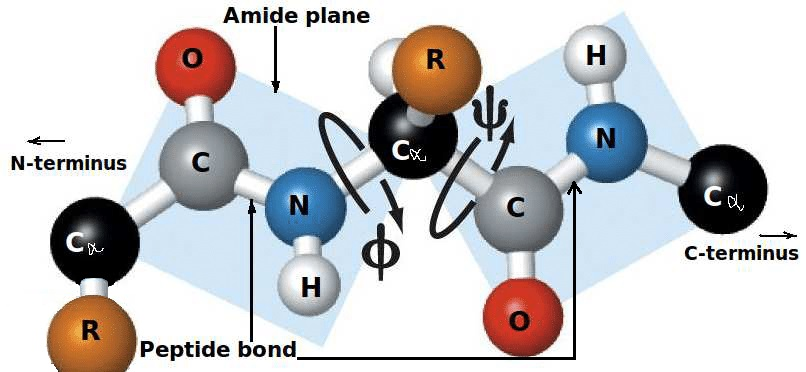
\includegraphics[scale=0.6]{res/dev/alphacarbon.png}
    \caption{$\alpha$-Carbon atoms in a protein}
    \label{fig:acarbons}
\end{figure}

$\alpha$-Carbon atoms are the core of residues, in the figure \ref{fig:acarbons} we can see them in a piece of a protein chain.

Now back to the P-SEA algorithm: for each residue i, we want to calculate these distance measures:
\begin{itemize}
    \item d2i: it's the distance between the residue (i-1) and the residue (i+1);
    \item d3i: it's the distance between the residue (i-1) and the residue (i+2);
    \item d4i: it's the distance between the residue (i-1) and the residue (i+3);
\end{itemize}

And these angle measures:
\begin{itemize}
    \item $\tau$i: the angle formed by the residues (i-1), i and (i+1);
    \item $\alpha$i: the dihedral angle formed by the residues (i-1), i, (i+1) and (i+2).
\end{itemize}

Distances and angles are computed between the $\alpha$-carbons of bonded residues.
Specific range of values in d2, d3, d4, $\tau$i, $\alpha$i determine in which secondary structure that residue falls into, among the main three categories:
\begin{itemize}
    \item \textbf{Helices};
    \item \textbf{Strands}: such as beta-sheets parallel and anti-parallel;
    \item \textbf{Coils}: turns and loops;
\end{itemize}

The thresholds for belonging in one of the two non coil secondary structure are shown in the table \ref{tab:thr-psea}.

\begin{table}[h!]
    \centering
    \begin{tabular}{|c|c|c|}
    \hline
        Parameters & Helix & Strand \\
    \hline
        Angle $\tau$ (\textdegree) & 89\hspace{0.3em} $\pm$\hspace{0.3em} 12 & 124\hspace{0.3em} $\pm$\hspace{0.3em} 14 \\
        Dihedral angle $\alpha$ (\textdegree) & 50\hspace{0.3em} $\pm$\hspace{0.3em} 20 & -170\hspace{0.3em} $\pm$\hspace{0.3em} 45 \\
        & & \\
        Distance d2 (\AA) & 5.5\hspace{0.3em} $\pm$\hspace{0.3em} 0.5 & 6.7\hspace{0.3em} $\pm$ \hspace{0.3em} 0.6\\
        Distance d3 (\AA) & 5.3\hspace{0.3em} $\pm$ \hspace{0.3em} 0.5 & 9.9\hspace{0.3em} $\pm$ 0.9 \\
        Distance d4 (\AA) & 6.4\hspace{0.3em} $\pm$ \hspace{0.3em} 0.6 & 12.4\hspace{0.3em} $\pm$ \hspace{0.3em} 1.1\\
        \hline
    \end{tabular}
    \caption{Parameters for P-SEA assignment of secondary structure.}
    \label{tab:thr-psea}
\end{table}

\begin{figure}[h!]
    \centering
    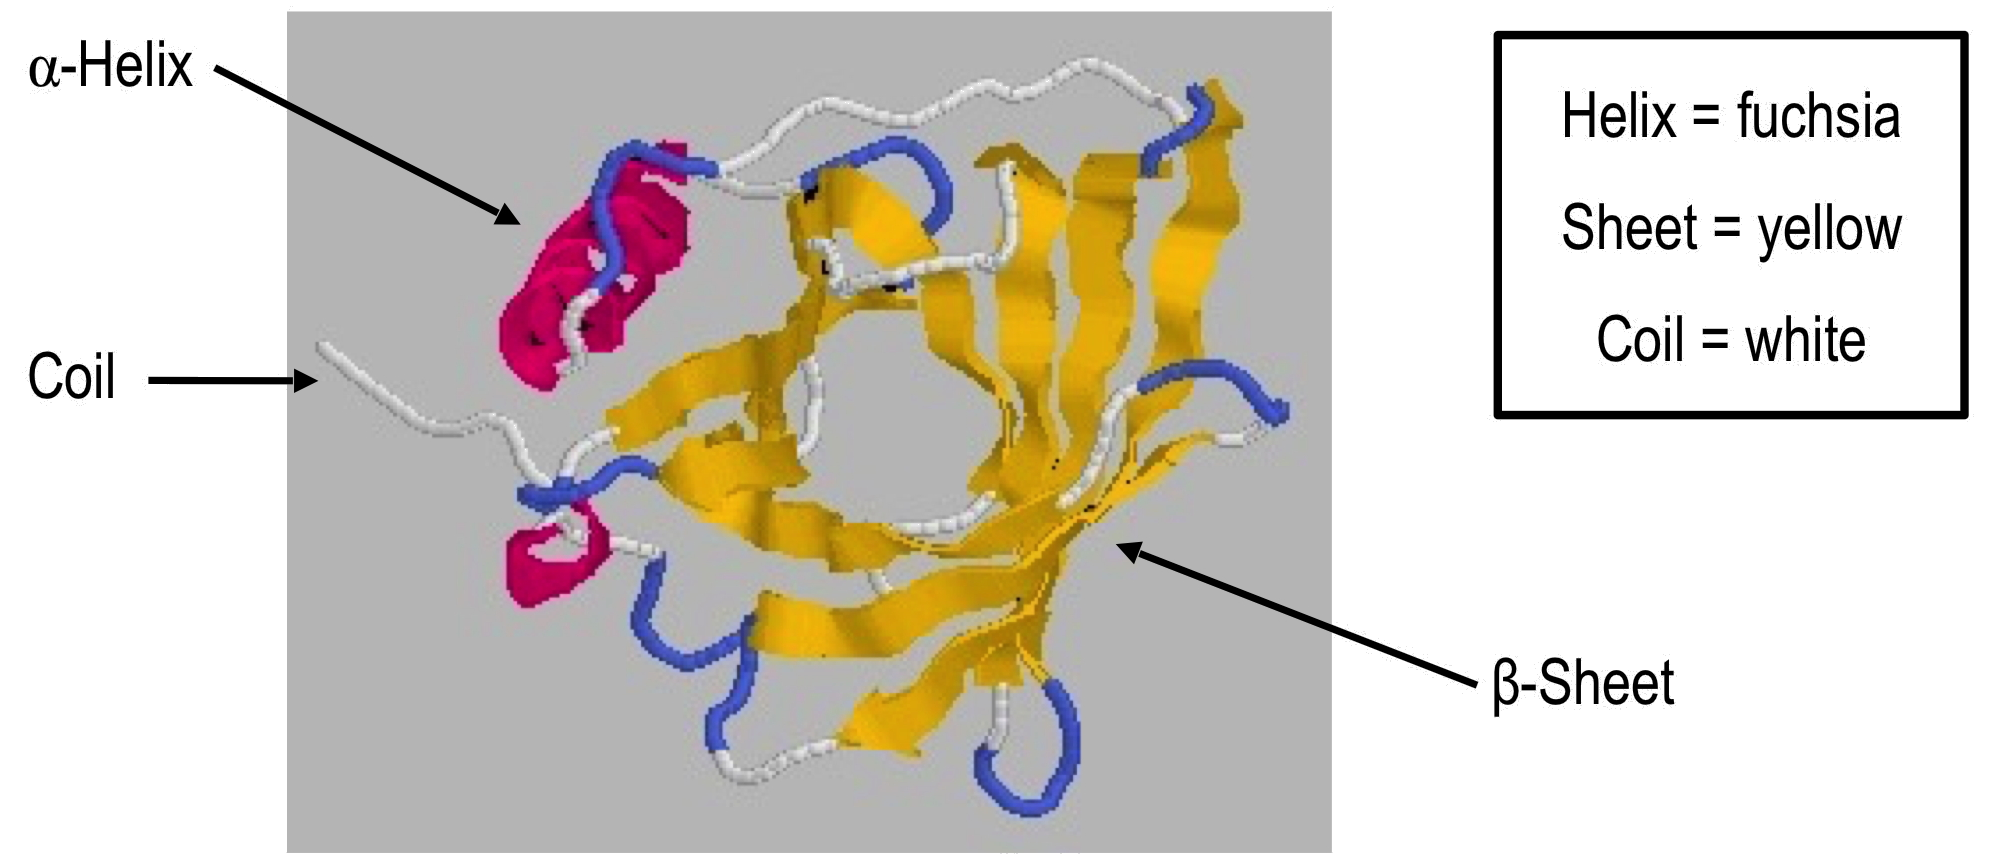
\includegraphics{res/dev/coil.png}
    \caption{The threee secondary structure P-SEA can identify}
\end{figure}

Let's see how we implemented the idea of algorithm discussed on the paper\cite{psea}.

\pagebreak

\subsection{Implementation of PSEA procedure}
Let's explore how we implemented the PSEA algorithm in a procedure.
Let's first analyze the various steps required from the algorithm:
\begin{enumerate}
    \item Get the coordinates of the residue's $\alpha$-carbon atom, for each residue in the protein;
    \item Compute distances and angles for each residue, as described in the paper;
    \item Assign to each residue it's secondary structure, based on computed distances and angles.
\end{enumerate}
We will analyze these steps one by one in this section.

\subsubsection{Get $\alpha$-carbon atom's coordinates for each residue}
In this first step we want to obtain the list of residues in the protein and then for each residue we want the coordinates of its $\alpha$-carbon.

We store them in a matrix with 3 columns and as many rows as the number of residues. In each row we store the 3 coordinates of the $\alpha$-carbon atom.

The basic idea would be to:
\begin{itemize}
    \item Obtain the list of atoms from the protein chain; 
    \item Obtain the list of $\alpha$-carbon atoms from the whole list of atoms;
    \item For each $\alpha$-carbon atom, obtain its residue with the BioPython function "get\_parent()";
    \item Store the coordinates of that $\alpha$-carbon atom in the row of that residue, in the matrix.
\end{itemize}

\begin{algorithm}[ht]
    \caption{Pseudocode for extracting $\alpha$-carbons coordinates}\label{alg:two}
    \begin{algorithmic}
        \REQUIRE{$struct$, a protein structure}
        \STATE list\_atoms = struct.get\_atoms()
        \STATE res\_start\_ids = get\_res\_start()
        \STATE list\_ca = empty list of size "len(res\_start\_ids)"
        \FOR{atom in list\_atoms}
            \IF{atom.name = "CA"}
                \STATE list\_ca.append(atom)
            \ENDIF
        \ENDFOR
        \STATE matrix\_coordinates = empty matrix of size "len(res\_start\_ids) x 3"
        \COMMENT{Res start ids are long the number of residues in the protein chain, and 3 because we have 3 coordinates: x,y,z.}
        \FOR{ca in list\_ca}
            \STATE matrix\_coordinates.append(ca.coordinates)
        \ENDFOR
    \end{algorithmic}
\end{algorithm}

This is the basic pseudo-code for this step. Although internally, the code is more optimized for computational purposes: we used NumPy methods to use the residues starting indexes more efficiently to create the $\alpha$-carbon coordinates' matrix.

\pagebreak

\subsubsection{Compute distances and angles between $\alpha$-carbon atoms}
Now we have a list of $\alpha$-carbon atoms, with their coordinates. The next step described in the paper is computing distances and angles between these atoms, to assign the correct secondary structure.

For each row of the matrix, which represent the residue's $\alpha$-carbon atom, compute the 5 measures:
\begin{itemize}
    \item \textbf{d2}: distance between atom at row i and atom at row i+2;
    \item \textbf{d3}: distance between atom at row i and atom at row i+3;
    \item \textbf{d4}: distance between atom at row i and atom at row i+4;
    \item angle $\tau$: angle between three consecutive atoms: at rows i, i+1 and i+2;
    \item angle $\alpha$: angle between four consecutive atoms: at rows i, i+1, i+2 and i+3.
\end{itemize}

I will show with a few pictures what distances and those 2 angles looks like, in the case of 5 consecutive $\alpha$-carbons. 

For simplicity the $\alpha$-carbon are directly linked, but in reality they have a lot of atoms between them, atoms that aren't $\alpha$-carbon.

Let's start from the angle $\tau$.

\begin{figure}[h!]
    \centering
    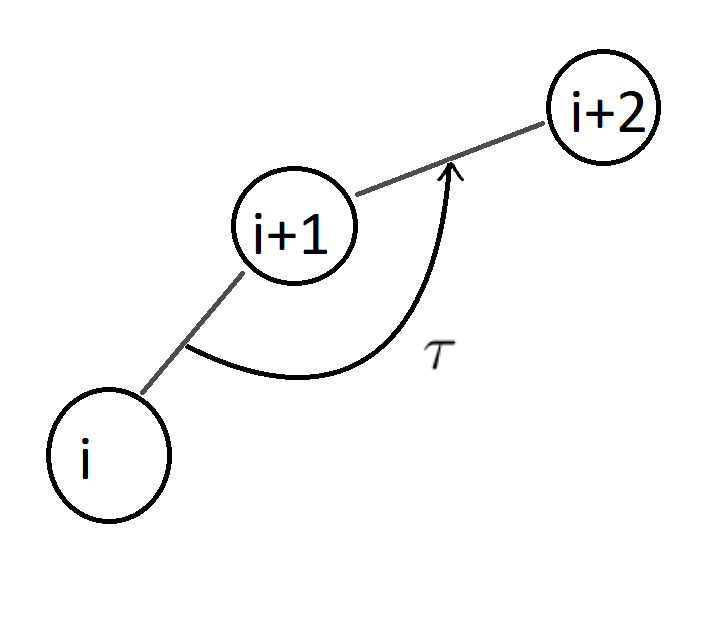
\includegraphics[scale=0.5]{res/dev/angleTau.png}
    \caption{Angle $\tau$}
\end{figure}

\pagebreak

And then we have the 3 distances: d2, d3 and d4.

\begin{figure}[h!]
    \centering
    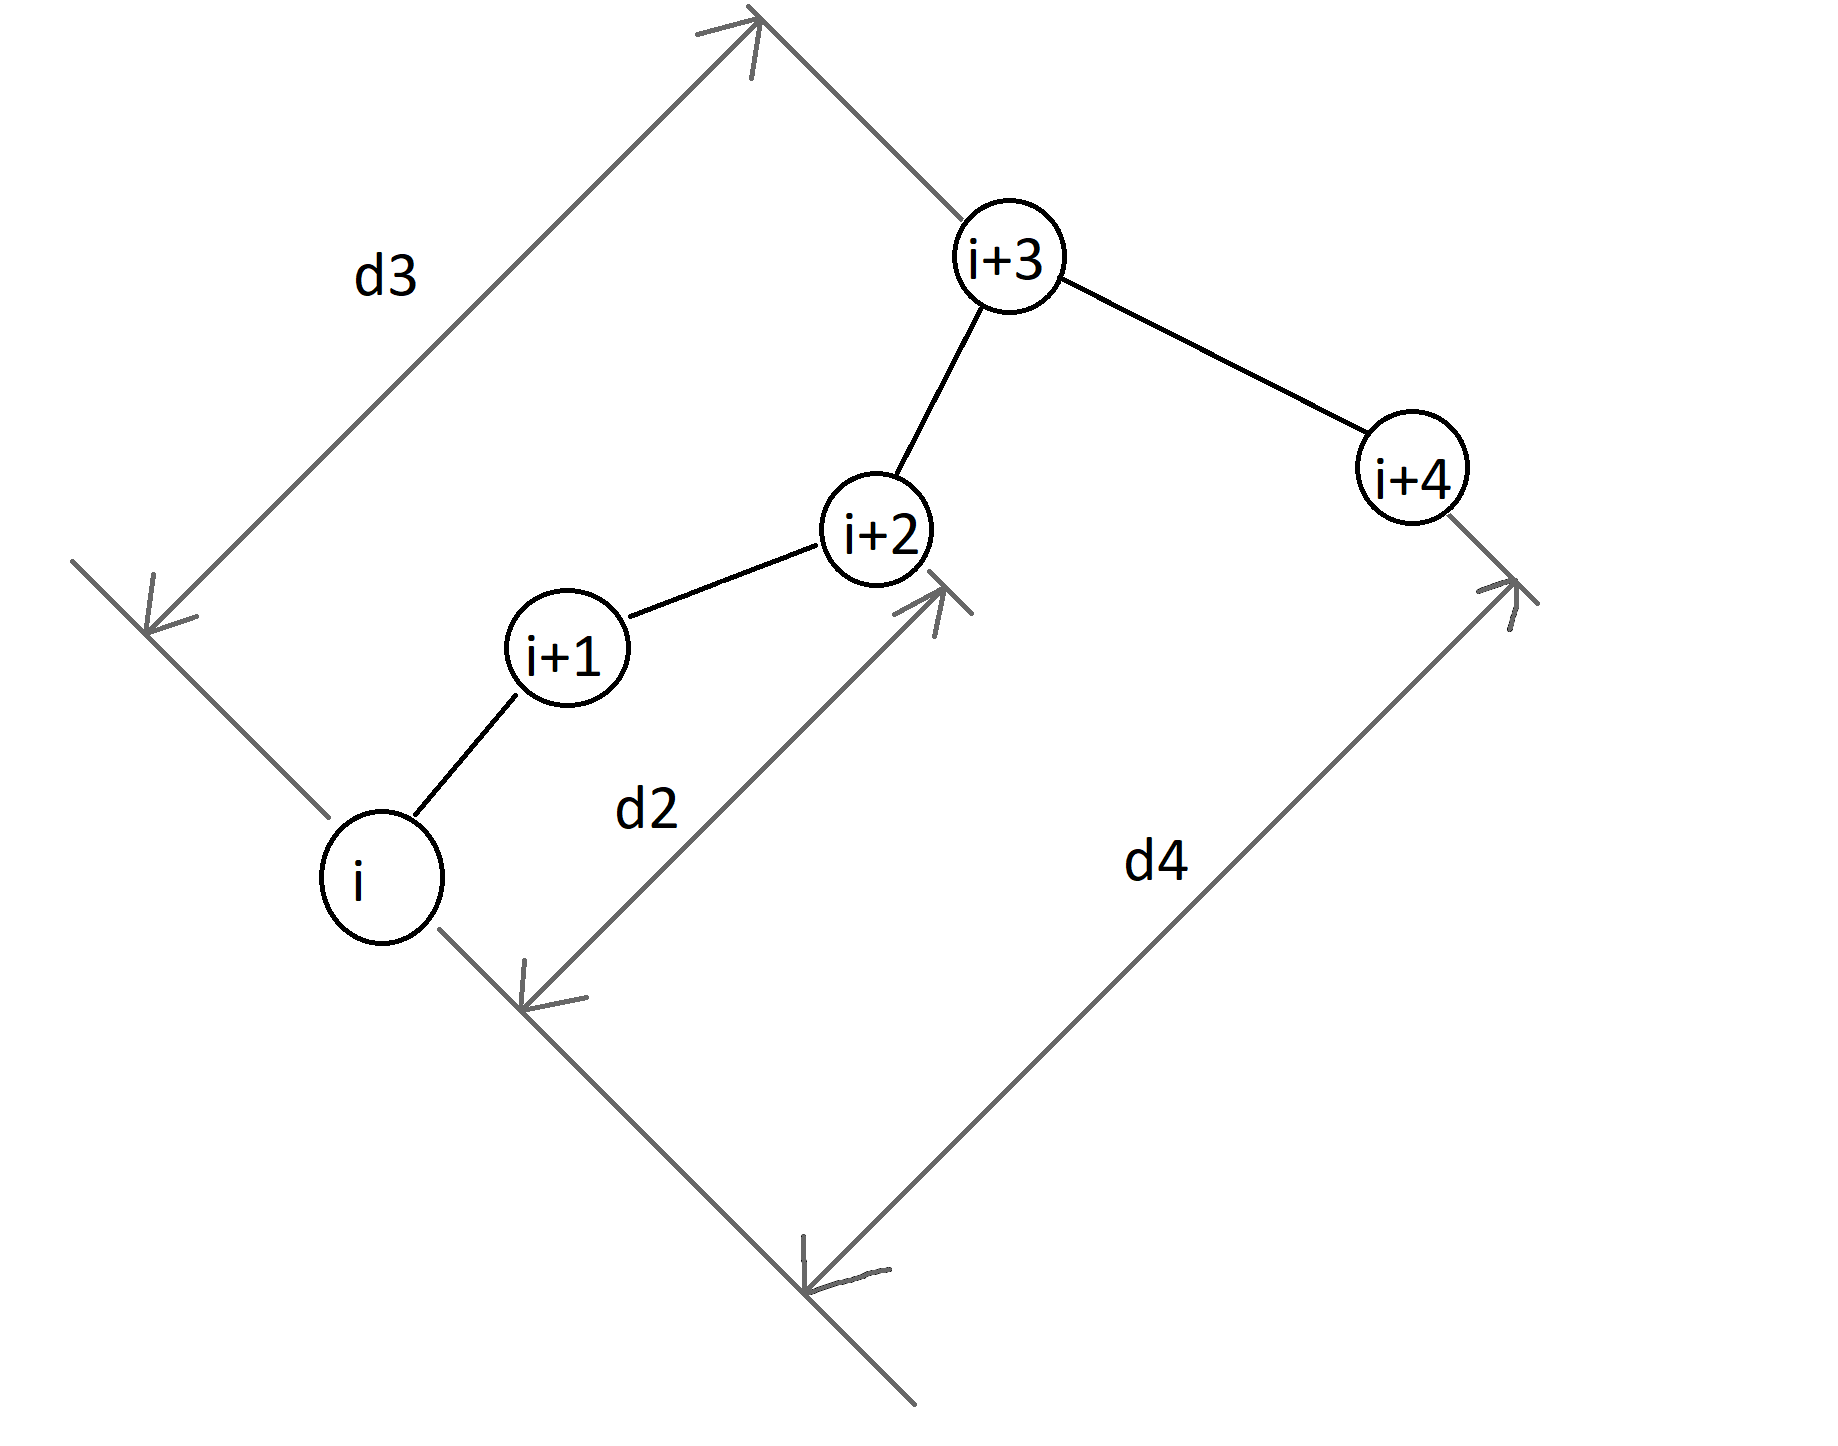
\includegraphics[scale=0.4]{res/dev/distances.png}
    \caption{Distances d2, d3 and d4}
    \label{fig:enter-label}
\end{figure}

\pagebreak
And finally the dihedral angle, the angle $\alpha$.

\begin{figure}[h!]
    \centering
    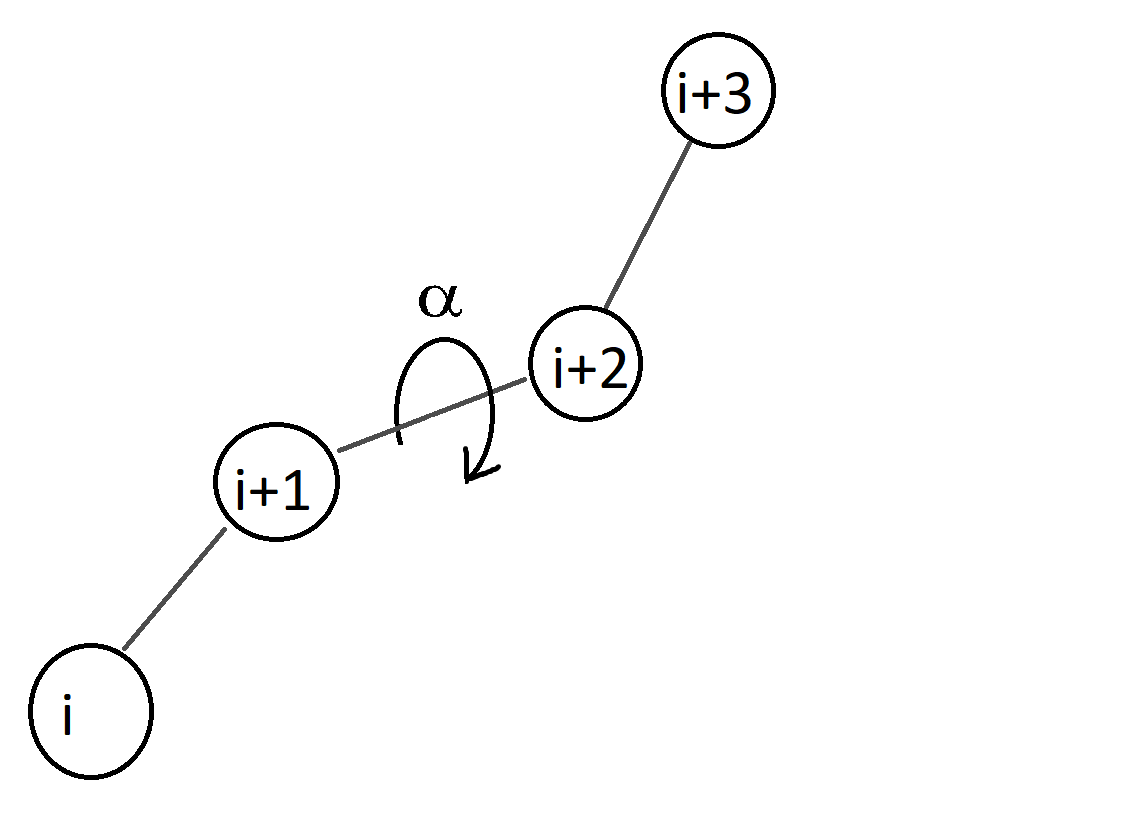
\includegraphics[scale=0.5]{res/dev/angleAlpha.png}
    \caption{Angle $\alpha$}
    \label{fig:enter-label}
\end{figure}

Now let's explore how we computed these measures:
\begin{itemize}
    \item \textbf{Distances}: for the distances we just use the euclidean norm, which is \\ {$||x||_2 = \sqrt{x_1^2 + ... + x_n^2}$}
    \item \textbf{Angle $\tau$}: for this angle we used the following formula \\ $\tau = arccos(\frac{a \cdot b}{||a|| \cdot ||b||})$. With $a = (v_{i+1}-v_i)$ and $b = (v_{i+1}-v_{i+2})$.  
    \item \textbf{Angle $\alpha$}: to calculate the dihedral angle between the 4 data points we have to calculate the angle between the two half-planes defined by three consecutive points. The first semi-plane $n_1$ is defined by the points $v_i$, $v_{i+1}$ and $v_{i+2}$. The second semi-plane is defined by the points $v_{i+1}$, $v_{i+2}$ and $v_{i+3}$.

    \pagebreak

    \begin{enumerate}
            \item We computed the vectors u,v and w by vector subtraction: $a = \frac{v_{i+1}-v_i}{||v_{i+1}-v_i||}$, $b = \frac{v_{i+2}-v_{i+1}}{||v_{i+2}-v_{i+1}||}$ and $c = \frac{v_{i+3}-v_{i+2}}{||v_{i+3}-v_{i+2}||}$;
            \item We computed the two half-planes $n_1 = a \times b$ and $n_2 = b \times c$ \footnote{This $\times$ symbol is to indicate the cross product between two vectors, while the $\cdot$ symbol is for dot product. More information on the cross product \href{https://en.wikipedia.org/wiki/Cross\_product}{\underline{here}.}};
            \item Finally we obtain the angle as $\alpha = arctan2((n_1\times n_2)\cdot b,\ n_1\cdot n_2)$.
    \end{enumerate}
\end{itemize}

Here we can see the pseudo-code to compute distances and angles.

\begin{algorithm}[ht]
    \caption{Pseudocode for computing angles and distances between $\alpha$-carbons coordinates}\label{alg:two}
    \begin{algorithmic}
        
        \REQUIRE{$ca\_coord$, a matrix containing the coordinates of the various $\alpha$-carbon atoms}
        \STATE d2 = \textbf{distance\_atoms}(ca\_coords[:-2], ca\_coords[2:])
        \STATE d3 = \textbf{distance\_atoms}(ca\_coords[:-3], ca\_coords[3:])
        \STATE d4 = \textbf{distance\_atoms}(ca\_coords[:-4], ca\_coords[4:])
        \STATE tau = \textbf{angle}(ca\_coords[:-2], ca\_coords[1:-1], ca\_coords[2:])
        \STATE alpha = \textbf{dihedral}(ca\_coords[:-3],ca\_coords[1:-2],ca\_coords[2:-1],ca\_coords[3:-2])
    \end{algorithmic}
\end{algorithm}

As we can see from the pseudo-code we used the python language built-in functions to compute all distances and angles in oneshot, but it's possible to implement it with of for loops.

\subsubsection{Assign secondary structure to each residue}
For this last step, we want to compute which residue belongs to a helix structure and which residue belongs to a strand structure.
The paper describes the procedure to assign to a residue the secondary structure, based on distances and angles, using the table for criteria: table \ref{tab:thr-psea}.

For assigning residues to helical structure:
\begin{itemize}
    \item Helices are first assigned to any segment long at least five residues, satisfying either one of the following helical criteria:
        \begin{enumerate}
            \item Each residue's $\alpha$-carbon in the segment satisfies both the helical criteria for d3i and for d4i distances;
            \item Each residue's $\alpha$-carbon in the segment satisfies both the helical criteria for $\alpha$i and $\tau$i angles.
        \end{enumerate}
    \item Then each of this segment is lengthened by one residue at each end and if those 2 residues satisfies some criteria we assign them to helix structure too. The criteria is that the residue satisfies either:
    \begin{enumerate}
        \item d3i distance helical criteria;
        \item $\tau$i angle helical criteria.
    \end{enumerate}
\end{itemize} 
Regarding the assigment of strand structure to residues, the procedure is similar:
\begin{itemize}
    \item Strand structure is assigned to any segment long at least three residues, satisfying either one of the following strand criteria:
    \begin{enumerate}
        \item Each residue's $\alpha$-carbon in the segment satisfies both the d2i, d3i and d4i distances criteria; 
        \item Each residues's $\alpha$-carbon in the segment satisfies both the $\tau$i and $\alpha$i angles criteria.
    \end{enumerate}
    \item Then lengthening by one residue at each end if it satisfies the d3i distance strand criteria;
    \item Finally short $\beta$-strand (<4 residues) are kept only if they have enough contacts, which means they are included in a $\beta$-sheet.
\end{itemize}

\begin{algorithm}[ht]
    \caption{Pseudocode for assigning secondary structure to residues}\label{alg:two}
    \begin{algorithmic}
        \REQUIRE{ca\_coords, d2, d3, d4, $\alpha$, $\tau$}

        \STATE basic\_helix = (d3 $\in$ (4.8, 5.8) AND d4 $\in$ (4.8, 7)) OR ($\tau \in$  (75, 101) AND $\alpha \in$ (30, 70))
        \STATE basic\_helix = \textbf{mask\_consecutive}(basic\_helix, 5)
        \STATE extended\_helix = \textbf{extend\_region}(basic\_helix)
        \STATE basic\_strand = (d3 $\in$ (4.8, 5.8) AND d4 $\in$ (4.8, 7)) OR ($\tau \in$  (75, 101) AND $\alpha \in$ (30, 70))
        \STATE basic\_strand = \textbf{mask\_consecutive}(basic\_strand, 3)
        \STATE extended\_strand = \textbf{extend\_region}(basic\_helix)
        \STATE extended\_strand = \textbf{mask\_regions\_with\_low\_contacts}(extended\_strand)

        \STATE ss\_prediction = list long len(ca\_coords) initialized with all "C"
        \STATE ss\_prediction[extended\_helix] = "H"
        \STATE ss\_prediction[extended\_strand] = "E"

    \end{algorithmic}
\end{algorithm}

\pagebreak

The procedures used in this pseudocode will be described later on in their section \ref{subsect:helper-procedures}:
\begin{itemize}
    \item \textbf{extend\_region};
    \item \textbf{mask\_consecutive};
    \item \textbf{mask\_regions\_with\_low\_contacts}.
\end{itemize}

After this step every residue will have its secondary structure assigned:
\begin{itemize}
    \item \textbf{H} for helix structure residues;
    \item \textbf{E} for strand structure residues;
    \item \textbf{C} for coils;
    \item \textbf{''} for residues without the $\alpha$-carbon.
\end{itemize}

\subsection{Helper procedures} \label{subsect:helper-procedures}
In this section we will describe more in detail the helper procedures used for the PSEA algorithm:
\begin{itemize}
    \item \textbf{get\_res\_start()}: procedure that creates a list of atoms out of the protein structure and then computes the start of each residues, by changes of residue name, id or chain id. It's possible to pass as parameter to the procedure "move\_hhem\_to\_end = True", this puts those atoms between chains to the end of the atom array, resulting in an higher accuracy of prediction of secondary structure in multi-chain proteins.
    \item \textbf{distance\_atoms()}: computes the distance between two atoms;
    \item \textbf{angle()}: computes the angle between three atoms;
    \item \textbf{dihedral()}: computes the dihedral angle between four atoms, between their semiplanes;
    \item \textbf{mask\_consecutive()}: this procedure is used to create the first step of helix and strand mask, where we want at least a segment of 3/5 residues satisfying a certain condition. It uses binary masks along with the library NumPy;
    \item \textbf{extend\_region()}: this procedure is for the second step of finding if a residue belong to that structure, which is lengthening. This procedure lengthen the segment if the residues satisfy the necessary criteria;
    \item \textbf{mask\_regions\_with\_low\_contacts()}: finally this procedure is used in the strand structure mask, short strands are kept only if they have enough contacts. This procedure "removes" from the strand masks, short strands with low contacts.
\end{itemize}

I decided to not show the code snippets for these procedures because they are complex and not too useful to understand the code, but they can be found in the \href{https://github.com/EvilCrive/AlphaFold-disorder/tree/MobiDB-Alphafold}{\underline{github repository}} in the file "utils\_alphafold\_disorder.py".

\subsection{Integration}
For the integration with the existing AlphaFold-disorder software tool, we encapsulated this psea algorithm in a procedure called get\_sse\_psea() which takes as input the protein structure and return as output an array of characters, with the secondary structure of each residue.
And the procedure called from the software-tool for each protein file is called "process\_pdb\_psea()". Based on which method we want to use there is a "process\_pdb\_psea()" procedure and a "procedure\_dssp()" one.

So the existing code isn't too much touched, since the only difference is that it has to call this procedure instead of the DSSP wrapper procedure.

Down below a code snippet of this procedure encapsulating the whole PSEA algorithm.

\begin{lstlisting}[language=Python, caption=Procedure get\_sse\_psea(), numbers=left]
def get_sse_psea(structure, add_short_contacts = True, move_end_hhem = True) :
    res_start_id, atom_array = get_res_start(structure, 
        move_end_hhem)
    ca_coord, novirtual_mask = get_ca_coord(res_start_id, atom_array)
    length, [d2i, d3i, d4i, ri, ai] = calc_dist_angles(ca_coord)
    helix_mask, strand_mask = calc_struct_mask(ca_coord, length, 
        [d2i, d3i, d4i], [ri, ai], add_short_contacts)
    
    return finalize_sse(ca_coord, length, novirtual_mask, 
        helix_mask, strand_mask)
        
\end{lstlisting}

We already talked about the procedures \textbf{get\_res\_start}, while \textbf{get\_ca\_coord}, like the name suggests creates the matrix of $\alpha$-carbon coordinates, \textbf{calc\_dist\_angles} is the procedure for computing the distances and angles. \textbf{calc\_struct\_mask} is the procedure to compute the helix mask and strand mask, this procedure takes as parameter "add\_short\_contacts", which if set to true removes short strands with low contacts.

And finally the \textbf{finalize\_sse} procedure uses the helix and strand masks to assign the secondary structure to each residue and returns an array of characters, each character representing the secondary structure for the residue at that array position.

We compared the secondary structure predicted with this method and the secondary structure predicted with DSSP for a few hundred proteins and as the paper\cite{psea} of PSEA said we got an accuracy of around 80\%. 

To compare that we used a procedure called "compare\_sses" which compares the secondary structure elements predicted from DSSP with the secondary structure predicted with PSEA algorithm.

\begin{lstlisting}[language=Python, caption=Procedure to compare SSEs, numbers=left]
def compare_sses(sse, dssp) :
    sse_dssp = [dssp[i][2] for i in dssp]
         
    counter1 = 0
    counter2 = 0
    countersize = 0
    for (i,j) in zip(sse, sse_dssp) :
        if j in ['H','G','I'] : 
            j = 'a'
        elif j in ['B', 'E'] : 
            j = 'b'
        else : 
            j = 'c'
        if i == '': i = 'c'
 
        if i == j :
            counter1 += 1
        if i in ['a','b'] : i = 'p'
        if j in ['a','b'] : j = 'p'
        if i == j :
            counter2 += 1
        #else :
            #print(i,j)
        countersize+=1
    counter1 = counter1/countersize
    counter2 = counter2/countersize
    if counter1 == counter2 :
        return round(counter1,4)
    else :
        return [counter1/countersize, counter2/countersize]

\end{lstlisting}
\pagebreak

\section{Computation of RSA with Shrake-Rupley Algorithm}
Let's go on with the next algorithm we implemented: since we do not use DSSP for the secondary structure, we wanted to not use DSSP at all. The other reason why DSSP is used in AlphaFold-disorder is the RSA, relative solvent accessibility.

So we implemented an alternative way to compute the RSA, without the DSSP. This method is uses the Shrake-Rupley algorithm, to compute SASA, solvent accessible surface areas. This value is then transformed into the relative solvent accessibility with two rounds of normalization factors: first by using Sander's normalization factors, like in DSSP, and then by using an ad-hoc normalization factors we made to not have rsa values bigger than 1, obtained from a sample of two thousands proteins.

We can summarize the steps for implementing this procedure in 2 steps:
\begin{itemize}
    \item Implement Shrake-Rupley algorithm to obtain the SASA statistics, for each residue;
    \item Normalization to obtain RSA statistics: both with Sander and Rost's normalization factors, explained in their scientific paper \cite{Sander-Rost} and with our ad-hoc normalization factors.
\end{itemize}

\subsection{Implement Shrake-Rupley algorithm}
The Shrake \& Rupley algorithm consists in a "rolling ball" of radius equal to a solvent molecule, which estimates the surface of the target molecule.
This algorithm allows us to compute the SASA statistic (Solvent Accessible Surface Areas), more details can be found in the relative scientific paper\cite{ShrakeRupley}.

To implement this algorithm in our code we just imported the library "Bio.PDB.SASA" and used the provided class "ShrakeRupley", with its function "compute()". We used the class to create an object of type "ShrakeRupley" and then applied the function "compute()" passing as parameters the protein structure and the level "R", R stands for residue, so that we compute the SASA statistic for each residue. We used the default paramters for the class ShrakeRupley since they are the right parameters for water as solvent, but in case of a different solvent we might want to change them.

We will see a snippet of the code for this procedure in the section \ref{subsect:rsaCode}.

\subsection{Normalization}

These SASA values aren't relative at all, they can have really high values, up to 200 or more. We want to obtain a statistic that represents the relative surface accessibility, so we have to perform some kind of normalization. We applied two rounds of normalization factors:

\begin{itemize}
    \item \textbf{Sander and Rost's normalization factors}: these are factors for normalization developed by Sander and Rost, with the maximum values of ASA values (Accessible Surface Areas). To use them we import the library "Bio.Data.PDBData" which contains the dictionary "residue\_sasa\_scales", this dictionary provide the normalization factor for each residue, so we apply these normalization factors to the SASA value we obtained for each residue;
    \item \textbf{Ad-hoc normalization factors}: since after applying the Sander and Rost's normalization factors we still had RSA values bigger than 1, we designed another round of normalization factors. We took all the proteins from the DisProt database, which are 2547 proteins, computed the SASA values for each residue and divided them by the Sander and Rost's normalization factors obtaining the norm\_SASA values. With all these norm\_SASA values we built up a dictionary of ad-hoc normalization factors. Finally we divided the norm\_SASA values by these ad-hoc normalization factors and obtained the final RSA values.
\end{itemize}

After these 2 rounds of division by normalization factors we obtain the RSA values, within a range of [0,1], representing the percentage of surface accessibility for that residue.

Now for reference I will show the values of the 2 rounds of normalization factors as tables.
\vspace{10em}
\pagebreak
\begin{table}[h!]
    \begin{tabular}{ |c|c|c| }
        \hline
        \textbf{3 Letters AA} & \textbf{1 Letter AA} & \textbf{Normalization Factor} \\\hline
        Ala & A & 106 \\\hline
        Arg & R & 248 \\\hline
        Asn & N & 157 \\\hline
        Asp & D & 163 \\\hline
        Cys & C & 135 \\\hline
        Gln & Q & 198 \\\hline
        Glu & E & 194 \\\hline
        Gly & G & 84 \\\hline
        His & H & 184 \\\hline
        Ile & I & 169 \\\hline
        Leu & L & 164 \\\hline
        Lys & K & 205 \\\hline
        Met & M & 188 \\\hline
        Phe & F & 197 \\\hline
        Pro & P & 136  \\\hline
        Ser & S & 130 \\\hline
        Thr & T & 142 \\\hline
        Trp & W & 227 \\\hline
        Tyr & Y & 222 \\\hline
        Val & V & 142 \\\hline
    \end{tabular}
    \caption{Sander and Rost's normalization factors}
\end{table}
\pagebreak
\begin{table}[h!]
    \begin{tabular}{ |c|c|c| }
        \hline
        \textbf{3 Letters AA} & \textbf{1 Letter AA} & \textbf{Normalization Factor} \\\hline
        Ala & A & 1.713 \\\hline
        Arg & R & 1.280 \\\hline
        Asn & N & 1.476 \\\hline
        Asp & D & 1.435 \\\hline
        Cys & C & 1.551 \\\hline
        Gln & Q & 1.311 \\\hline
        Glu & E & 1.360 \\\hline
        Gly & G & 1.804 \\\hline
        His & H & 1.404 \\\hline
        Ile & I & 1.413 \\\hline
        Leu & L & 1.532 \\\hline
        Lys & K & 1.357 \\\hline
        Met & M & 1.420 \\\hline
        Phe & F & 1.434 \\\hline
        Pro & P & 1.490  \\\hline
        Ser & S & 1.515 \\\hline
        Thr & T & 1.507 \\\hline
        Trp & W & 1.423 \\\hline
        Tyr & Y & 1.346 \\\hline
        Val & V & 1.549 \\\hline
    \end{tabular}
    \caption{Ad-hoc normalization factors}
\end{table}

\pagebreak


\subsection{Integration} \label{subsect:rsaCode}

Regarding the integration into the exisiting software-tool AlphaFold-disorder, we implented this algorithm for RSA inside the procedure "process\_pdb\_psea" since it's an alternative way to compute rsa compared to the one in "process\_pdb\_dssp". 

For the normalization factors:

\begin{itemize}
    \item Sander's normalization factors: it's enough to import the dictionary "residue\_sasa\_scales" from "Bio.Data.PDBData", which contains the normalization factors of each residue;
    \item Ad-hoc normalization factors: we created a file .json called "dict\_max\_rsa.json", which contains the normalization factors of each residue.
\end{itemize}

Once we have the dictionary of the normalization factors, we can obtain the factor of our residue simply by obtaining the value paired with that residue in the dictionary.

Down below a code snippet of the implementation of this Shrake \& Rupley algorithm to obtain the RSA values.

\begin{lstlisting}[language=Python, caption=Integration of rsa with SASA on process\_pdb\_psea procedure]
def process_pdb_psea(pdb_file, pdb_name) :
    structure, real_file = extract_pdb(pdb_file)
    with open('dict_max_rsa.json','r') as f :
        dict_adhoc_factors = json.load(f)
[...]
    sse = get_sse_psea(structure)
[...]
    ShrakeRupley().compute(structure, level="R")
    for i, residue in enumerate(structe.get_residues()):
[...]
        rsa = residue.sasa / residue_sasa_scales['Sander'][residue.resname]
        rsa = rsa / dict_adhoc_factors[protein_letters_3to1[residue.resname]]
[...]
\end{lstlisting}

\pagebreak

\section{Implementation of FoldComp Library}
We used the library FoldComp, described in more detail in their scientific paper \cite{foldcomp}, to allow to use a new input file in the software tool.

With FoldComp we can read and write .fcz file, which are compressed protein files, this enable us to store more protein files in the same storage space.

Regarding the implementation, we have:
\begin{itemize}
    \item "\textbf{decompress}" procedure of FoldComp;
    \item we made a procedure for checking if a file is a .fcz file "\textbf{is\_fcz\_file}": if the file starts with \textit{b'FCMP:'}, then it's a .fcz file.
\end{itemize}
Since in our case we are interested just in reading files .fcz we just need the procedure "decompress" from the library, which decompress the .fcz file into a .pdb file.

We also used the library \textbf{StringIO} as a workaround to avoid saving the protein file after decompressing the .fcz file.

Let's see the integration of this library into the software-tool AlphaFold-disorder.

\begin{lstlisting}[language=Python, caption=Integration of FoldComp]
def is_fcz_file(filepath) :
    with open(filepath, 'rb') as test_f:
        return test_f.read(5) == b'FCMP:'

def extract_pdb(pdb_file) :
[...]
    elif is_fcz_file(real_file):
        with open(real_file, 'rb') as f :
            (name, pdb_filevalue) = foldcomp.decompress(f)
        structure = PDBParser(QUIET=True).get_structure('', StringIO(pdb_filevalue))
[...]
\end{lstlisting}
